\documentclass[10pt,a4paper]{article}
\usepackage[margin=2.1cm]{geometry}
\usepackage{booktabs}
\usepackage{graphicx}
\usepackage{xcolor}
\usepackage{listings}
\usepackage{caption}
\usepackage{float}
\usepackage{hyperref}
\usepackage{amsmath}
\hypersetup{colorlinks=true, linkcolor=blue!60!black, urlcolor=blue!60!black}
\captionsetup{font=small, labelfont=bf}
\lstset{basicstyle=\ttfamily\scriptsize, breaklines=true, frame=single,
  framesep=4pt, xleftmargin=4pt, commentstyle=\color{gray}, columns=fullflexible}

\newcommand{\good}[1]{\textcolor{green!55!black}{#1}}
\newcommand{\bad}[1]{\textcolor{red!75!black}{#1}}
\newcommand{\warn}[1]{\textcolor{orange!85!black}{\textbf{#1}}}

\title{Function-eval grading report:\\experiment 08 vs.\ base under jac 0.36.1}
\author{jac-data-gen \texttt{evals/function/v1}, test split (1000 tasks)}
\date{Graded 2026-09-16 \;\textperiodcentered\; analysis of \texttt{fn\_eval\_preds/}}

\begin{document}
\maketitle
\vspace{-2.2em}

\section*{Executive summary}

\begin{itemize}
  \item \textbf{The LoRA (08) works.} Same 1000 tasks: the adapter lifts pass@1 from
        \bad{0/1000} (base) to \good{219 passes}, and compile rate from 5.9\% to
        \good{73.7\%}. It also taught contract discipline: 99.7\% of 08 outputs stay inside
        the feature contract vs.\ 59.2\% for base.
  \item \textbf{But the 08 grade is not trustworthy as printed.} The grading machine ran
        out of disk mid-run: 251 tasks are marked \texttt{infra\_error} (grader exit 2,
        run incomplete), and another \warn{59 ``test\_fail'' rows are really
        ``postgres failed to start''} infra errors that the grader's infra regex missed.
        Corrected: \textbf{310 of 1000 tasks (31\%)} were infra-killed, not model failures.
  \item \textbf{On cleanly-graded tasks 08 scores 31.7\% pass@1} (219/690). Projecting the
        infra tasks at the same compile-conditional rates gives an estimated
        \textbf{33--37\%} for a complete run --- i.e.\ the reported 29.2\% understates the model.
  \item \textbf{Translation is the adapter's strong track} (50.2\% pass, 78.7\% compile);
        completion is weak (15.0\% pass, 46.5\% compile), mostly because the model
        truncates or malforms the provided prefix (75\% of completion check-fails).
  \item \textbf{jac 0.36.1 grading itself is non-deterministic.} Re-grading 12 sample tasks
        on a healthy disk flipped 2 of 2 pass-controls to test\_fail --- the same code
        passes via the \emph{native} path but fails via the \emph{server codespace} path
        (e.g.\ \texttt{E1053} type errors that only fire in the server runtime).
        All 3 check-fail controls reproduced exactly. Passes are lucky rolls;
        treat every pass@1 from this toolchain as an upper bound.
  \item \textbf{Base fails in a characteristic way:} 0/500 compilable translations ---
        it writes \emph{old-Jac syntax} (\texttt{func f(..): T}) that the 0.36.1 parser
        rejects (72\% of all its check-fails), plus degenerate repetition loops that
        break extraction on 124 completion tasks.
\end{itemize}

\begin{figure}[h]
\centering
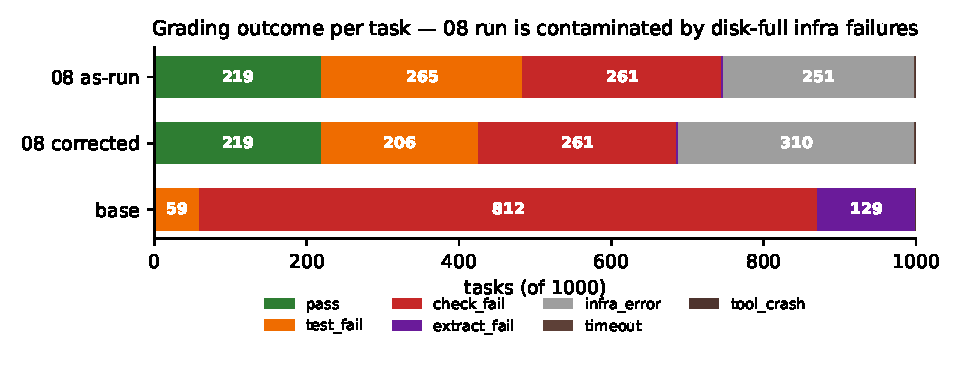
\includegraphics[width=.98\textwidth]{c1_status.pdf}
\caption{Outcomes for all 1000 tasks. ``08 corrected'' reclassifies 59 postgres-startup
failures from \texttt{test\_fail} to \texttt{infra\_error}. Base's 9 hidden infra failures
are shown in the base bar too (see \S\ref{sec:infra}).}
\end{figure}

\section{Setup}

Two systems answered the same 1000 tasks (500 \emph{completion}: finish a partly written
Jac function from a prefix; 500 \emph{translation}: port a Python function to Jac). Each
task hides Jac \texttt{test} blocks. A task \textbf{passes} only if the candidate
\begin{enumerate}
  \item yields a parseable \texttt{```jac} block (else \texttt{extract\_fail}),
  \item survives \texttt{jac check} (else \texttt{check\_fail}),
  \item passes every hidden test under \texttt{jac test} (else \texttt{test\_fail}), and
  \item keeps the feature contract (no Python syntax, no \texttt{import:py}, \ldots).
\end{enumerate}

\begin{itemize}
  \item \textbf{08} = Qwen3-Coder-30B-A3B (MLX 4-bit) + experiment-08 LoRA adapter.
  \item \textbf{base} = same model, no adapter.
  \item Grader: \texttt{eval\_jac.py} (jac-data-gen @ \texttt{5222202a}), 4 threads $\times$ 2
        pytest workers, 900\,s per stage, \textbf{jac 0.36.1} --- the toolchain the eval
        targets. The original experiment grade used 0.16.1.
\end{itemize}

\section{Headline numbers}

\begin{table}[h]
\centering\small
\begin{tabular}{lrrrrl}
\toprule
 & pass@1 & compile & contract & run & note \\
\midrule
08, as reported       & 29.2\% & 73.7\% & 99.7\% & incomplete & 251 infra; pass/749 eligible \\
08, corrected         & \good{31.7\%} & --- & --- & graded 690/1000 & 59 pg-fails moved to infra \\
08, projected full    & \good{$\sim$33--37\%} & --- & --- & estimate & see \S\ref{sec:projection} \\
base                  & \bad{0.0\%}  & \bad{5.9\%}  & \bad{59.2\%} & complete & 0/1000 pass \\
\midrule
\multicolumn{6}{l}{\emph{Reference: same preds under jac 0.16.1 (from README): 08 pass@1 57.0\%, base 3.0\%.}}\\
\bottomrule
\end{tabular}
\caption{Overall results. The 0.16.1 comparison is indicative only: that run used a
different parser/type-checker, and this run's 08 grade is contaminated (see \S\ref{sec:infra}).}
\end{table}

\section{Task breakdown}

\begin{figure}[h]
\centering
\begin{minipage}{.52\textwidth}
\centering
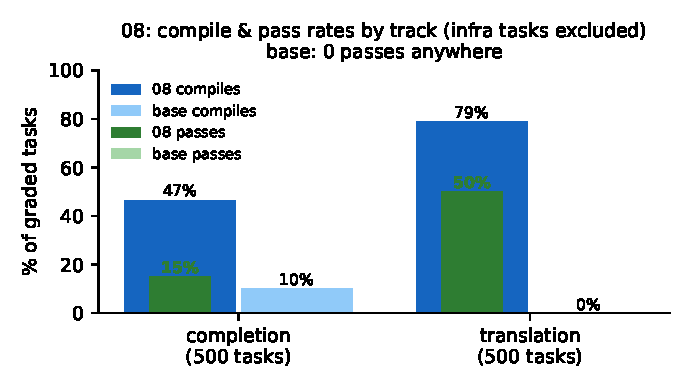
\includegraphics[width=\textwidth]{c2_tracks.pdf}
\end{minipage}\hfill
\begin{minipage}{.44\textwidth}
\centering\small
\begin{tabular}{lrr}
\toprule
08 (infra excluded) & compl. & transl. \\
\midrule
graded       & 361 & 329 \\
pass         & 54  & 165 \\
             & \good{15.0\%} & \good{50.2\%} \\
compiles     & 168 & 259 \\
             & 46.5\% & 78.7\% \\
check\_fail  & 191 & 70 \\
test\_fail   & 112 & 94 \\
extract\_fail& 2   & 0 \\
\bottomrule
\end{tabular}
\end{minipage}
\caption{08 by track. Translation --- the adapter's main gain: 3.3$\times$ the completion
pass rate. Completion fails early: 191/361 never even parse.}
\end{figure}

\subsection*{Where 08's check-fails come from}

\begin{figure}[H]
\centering
\begin{minipage}{.55\textwidth}
\centering
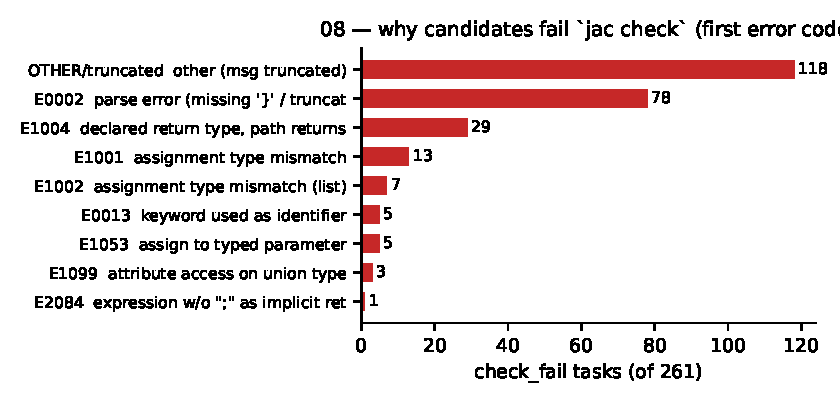
\includegraphics[width=\textwidth]{c3_codes.pdf}
\end{minipage}\hfill
\begin{minipage}{.42\textwidth}\small
Completion check-fails (191) are dominated by
\textbf{structural damage to the given prefix}: missing \texttt{\}} (E0002, 76) and
truncated/mangled output (88 whose message tail is cut before the code appears).
Translation check-fails (70) are \textbf{semantic}: the 0.36.1 type checker rejects
assignments and return paths that 0.16.1 accepted (E1001/E1002/E1053/E1099/E1004).
\end{minipage}
\caption{First error code per 08 check-fail.}
\end{figure}

\subsection*{Base: failure anatomy (all 1000 tasks fail)}

\begin{figure}[H]
\centering
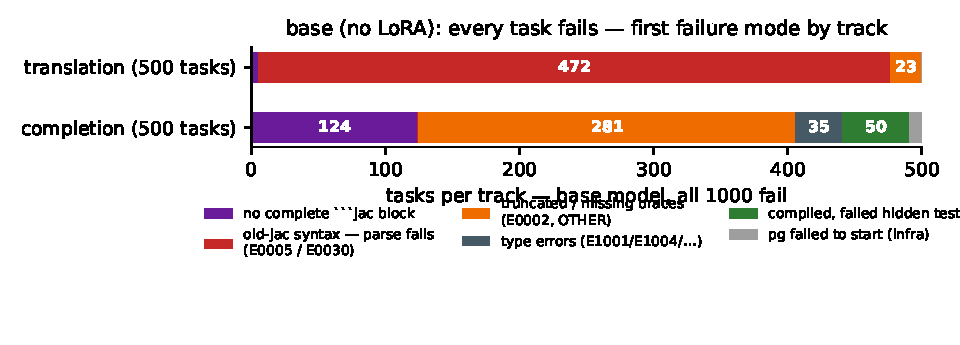
\includegraphics[width=.9\textwidth]{c5_base.pdf}
\end{figure}

Base never emits valid 0.36.1 Jac for translation: 472/500 die in the parser because it
writes pre-0.4 ``old Jac'' signatures, e.g.\ for \texttt{fn-translate-337455}:

\begin{lstlisting}
func _cmp(kd1: any, kd2: any): int {   # old syntax: colon return type
    ...
}
# -> E0005 Unexpected token 'return' ... E0030 Unexpected semicolon at module level
\end{lstlisting}

On completion tasks it loops: 379/1000 base responses contain degenerate line
repetition; when the loop swallows the closing fence the extractor gives up
(124 \texttt{extract\_fail}):

\begin{lstlisting}
```jac
    if k == 'registry' {
        return 'registry'
    }
    if k == 'registry' {        # ... repeated 40+ times, fence never closed
\end{lstlisting}

The 50 base completions that do compile still fail their hidden tests --- base's 3.0\%
pass@1 under 0.16.1 was already luck-level; under the stricter 0.36.1 checker it is 0.

\subsection*{What the LoRA actually taught}

\begin{table}[h]
\centering\small
\begin{tabular}{lrr}
\toprule
output statistic (1000 preds) & base & 08 \\
\midrule
opens translation fence with \texttt{```jac} & 99.0\% & 99.8\% \\
typed signatures (\texttt{typed\_def})       & 43.2\% & \good{99.3\%} \\
no Python-syntax smell                       & 68.1\% & \good{99.9\%} \\
inside feature contract                      & 59.2\% & \good{99.7\%} \\
new-style \texttt{def f(..) -> T \{ \}} on translation & \bad{$\sim$0\%} & \good{$\sim$100\%} \\
repetition-loop responses                    & 379 & 333 \\
\bottomrule
\end{tabular}
\caption{The adapter's job was mostly \emph{syntax and format normalization}: new-Jac
signatures, static types, no Python leakage. Base simply speaks the wrong dialect.}
\end{table}

\section{The 08 run is contaminated: infra forensics}
\label{sec:infra}

\textbf{1. Disk filled up during the run.} The first infra error appears at task
$\approx$267; from then on the run alternates between working windows and windows where
jac's embedded PostgreSQL cannot write (\texttt{PgWireError: \dots No space left on
device}) or cannot start at all. All 310 infra tasks had already passed
\texttt{jac check} and died in the test stage.

\textbf{2. The grader undercounts infra failures.} Its infra regex does not know the
\texttt{AssertionError: postgres failed to start: pg\_ctl: could not start server}
collection error, so 59 of those were recorded as ordinary \texttt{test\_fail}
(0 passes, 94 tasks graded in block 900+ --- all failures, zero passes).
Base's run, on a healthy disk, still hit 9 of the same pg-start failures --- the pg
startup is flaky under 4-way concurrency even with space free.

\textbf{3. A stale postmaster is still running.} A PostgreSQL started at 17:42 during the
run (PID 233078, socket \texttt{/tmp/jacpg-f4480dba16}) is alive and a stale lock in
\texttt{/tmp/jacpg-4f008fa8cc} blocks new \texttt{jac test} runs until cleaned.

\begin{figure}[h]
\centering
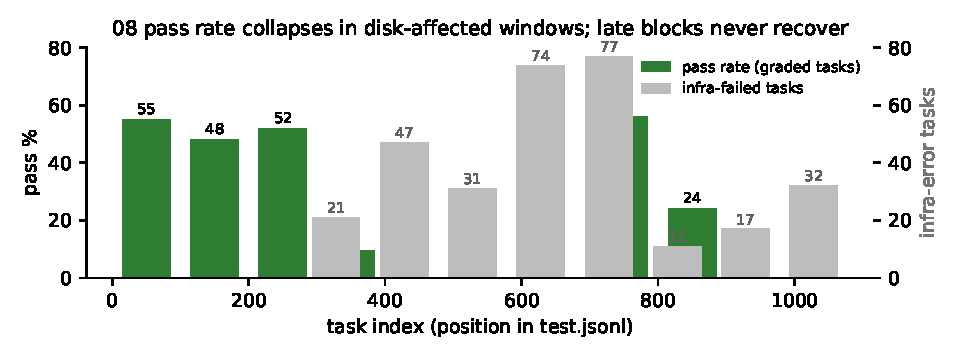
\includegraphics[width=.95\textwidth]{c4_blocks.pdf}
\caption{Pass rate per 100-task block (green, left axis) vs.\ infra-killed tasks (grey,
right axis). Windows with heavy infra damage score $\approx$0; clean windows recover to
50--56\% --- evidence the collapse is environmental, not model quality.}
\end{figure}

\subsection*{Projected score for a complete, clean run}
\label{sec:projection}

Infra tasks all compiled. Applying the clean compile-conditional pass rates
(completion 54/168 = 32.1\%, translation 165/259 = 63.7\%) to the 139 completion + 171
translation infra tasks projects $\approx$99 + 274 $\approx$ \textbf{373 passes} (37\%).
The conservative version (infra tasks at the unconditional graded rates) gives
$\approx$326 (33\%). Honest summary: \textbf{08's true score is between the corrected
31.7\% and $\approx$37\%, not the printed 29.2\%.}

\section{The grader is non-deterministic: re-run experiment}
\label{sec:regrade}

After freeing disk (35\,GB free), I re-graded 12 tasks (5 controls + 7 suspicious
failures) with the same binary, grader, and flags (\texttt{PYTEST\_XDIST\_AUTO\_NUM\_WORKERS=2}
had no effect on the outcome):

\begin{table}[h]
\centering\small
\begin{tabular}{lll}
\toprule
original status & re-grade status & count \\
\midrule
check\_fail & check\_fail (identical) & 3/3 \\
pass        & \bad{test\_fail}         & \bad{2/2 flipped} \\
test\_fail  & test\_fail               & 7/7 (but see below) \\
\bottomrule
\end{tabular}
\caption{Stability on re-grade.}
\end{table}

The two flipped tasks are the smoking gun. \texttt{fn-translate-337455} passed originally
and failed on re-grade with
\texttt{error[E1053]: Cannot assign dict[int, int] to parameter 'kd1' of type int | str}
--- its code annotates \texttt{kd1: int | str} but a hidden test calls
\texttt{\_cmp(\{2:1\}, \{2:1\})}. The other flipped on
\texttt{error[E5092]: Native lowering failed for builtin call 'min'}. Both messages carry
the note \emph{``preferred native but did not lower; compiled in the server codespace''}:
jac 0.36.1 runs tests through two different engines (native lowering vs.\ the
PostgreSQL-backed server runtime), they disagree on type strictness, and which engine
executes a given task varies run to run. \textbf{Consequences:} check\_fail verdicts are
trustworthy; individual passes are not reproducible; any pass@1 measured with this
toolchain is an upper bound on true functional correctness.

\section{Recommendations}

\begin{enumerate}
  \item \textbf{Re-run 08 end-to-end} on a machine with headroom; keep an eye on
        \texttt{df} mid-run, or cap concurrency (WORKERS=2) to reduce pg pressure.
  \item \textbf{Patch the grader's infra regex} to also match
        \texttt{postgres failed to start} / \texttt{pg\_ctl} / \texttt{PgWireError} so pg
        startup failures stop masquerading as model failures.
  \item \textbf{Before trusting passes, re-grade them once} and count only
        pass$\wedge$pass (or report best-of-2 and both-of-2). For training-signal
        purposes, treat reward from this grader as noisy-positive.
  \item \textbf{Clean up before the next run:} kill stale postmasters and remove
        \texttt{/tmp/jacpg-*} lock dirs.
  \item \textbf{Data-side lever for completion:} the dominant completion failure is
        structural damage to the prefix (E0002/truncation, 164 of 361 graded). More
        training pairs that \emph{copy the prefix verbatim and close all braces} is the
        cheapest win; translation is already at 50\% and mostly limited by the 0.36.1
        type checker (strictness 0.16.1 never applied).
\end{enumerate}

\section*{Appendix: artifacts}
\small
\begin{tabular}{ll}
\toprule
path & content \\
\midrule
\texttt{out/\{08,base\}/results.jsonl} & one row per task: status, error, static stats \\
\texttt{out/\{08,base\}/summary.json}  & grader aggregate \\
\texttt{out/\{08,base\}/grade.log}     & grader console output \\
\texttt{report/stats.json}            & every number in this report \\
\texttt{report/c*.pdf}                & figures \\
\texttt{/tmp/regrade*/results.jsonl}  & \S\ref{sec:regrade} re-run evidence \\
\bottomrule
\end{tabular}

\end{document}
